\documentclass[10pt]{article}
\usepackage[utf8]{inputenc}
\usepackage[T1]{fontenc}
\usepackage{amsmath}
\usepackage{amsfonts}
\usepackage{amssymb}
\usepackage{mhchem}
\usepackage{stmaryrd}
\usepackage{hyperref}
\hypersetup{colorlinks=true, linkcolor=blue, filecolor=magenta, urlcolor=cyan,}
\urlstyle{same}
\usepackage{graphicx}
\usepackage[export]{adjustbox}
\graphicspath{ {./images/} }

\title{Optimization of Optical Receiver Parameters for Pulsed Laser-Tracking Systems }


\author{Lazo M. Manojlović and Žarko P. Barbarić}
\date{}


\begin{document}
\maketitle


\begin{abstract}
Theoretical analysis and optimization of an optoelectronic receiving chain in pulsed laser-tracking systems are presented. The optical receiver and electronics for analog signal processing measure the angle displacements between the optical axis of the receiver and the direction optical receiver-designated object based on current signals that are generated on the avalanche quadrant photodiode. Considering the minimum allowed angle measurement error, the optimal optical receiver aperture diameter, the optimal size of the avalanche quadrant photodiode, and the maximal range of such a system are estimated.
\end{abstract}

Index Terms -Position-sensitive optical receiver (PSOR), pulsed laser-tracking system.

\section{INTRODUCTION}
’

T ODAY, pulsed laser systems are widely used in the field I of civil and maritime engineering, as well as for military purposes [1]. By using a pulsed laser designator and the corresponding optical receiver, some parameters of the laserilluminated object can be determined, such as the distance to the object and its angle displacements. The principle of distance and angle displacement measurements is based on laser pulse emission, which illuminates the object and whose parameters are to be determined, and their reception with the corresponding optoelectronic receiver [1]. After analog signal processing, the aforementioned parameters can be determined. By controlling the dynamic range of the received reflected optical radiation and using a well-designed analog signal processing chain, it is possible to reach an accuracy of several millimeters when measuring distances of several hundreds of meters. To measure angle displacements, instead of a standard photodiode, it is necessary to use an optical receiver, whose response depends on the light spot position on its surface. There are several types of such an optical receiver, but the quadrant photodiode and the lateraleffect photodiode are the most common [2]. The quadrant photodiode is almost exclusively used in pulsed laser-tracking systems because of its increased sensitivity and lower overall noise compared with the lateral-effect photodiode. Recently, the avalanche quadrant photodiode (AQPD) with good matching of

Manuscript received March 29,\(2008 ;\) revised August 2,2008 . First published

September 30,2008 ; current version published February 9,2009 .

L. M. Manojlović is with the Integrated Microsystems Austria \(\mathrm{GmbH}, 2700\) Wiener Neustadt, Austria (e-mail: \href{mailto:manojlovic@ima-mst.at}{manojlovic@ima-mst.at}).

Ž. P. Barbarić is with the Faculty of Technical Sciences, University of

Novi Pazar, 36300 Novi Pazar, Serbia (e-mail: \href{mailto:barbaric@etf.rs}{barbaric@etf.rs}).

Color versions of one or more of the figures in this paper are available online

at \href{http://ieeexplore.ieee.org}{http://ieeexplore.ieee.org}.

Digital Object Identifier 10.1109/TIM.2008.2005259 the segment avalanche amplification has been on the market. The advantage in using the \(A Q P D\) is that it has lower overall noise compared with the standard quadrant p-i-n photodiode.

The basic subject of this paper is the optimization of the optical and electronic receiver parameters for pulsed laser-tracking systems. The reflected optical radiation from the illuminated object is collected on the receiving optics. The received optical power levels, from the object and the background, mostly determine the characteristics of the pulsed laser-tracking system. Therefore, the estimations of the received optical powers are given in Section II. The position-sensitive optical detector consists of both the receiving optics and the analog signal processing chain, which are used for processing signals from the quadrant photodiode. A more detailed description of a positionsensitive optical receiver (PSOR) is given in Section III.

The most significant part of analog signal processing is the preamplifier. As an optimal solution for the preamplifier, the transimpedance amplifier (TIA) is used. In Section IV, the optimal transimpedance configuration for achieving the minimal overall noise in the receiving chain is presented. The equivalent input noise current was calculated as the optimal avalanche amplification of each avalanche photodiode.

Section \(\mathrm{V}\) shows how atmospheric turbulence influences the measurement precision. The angle-of-arrival fluctuations and illumination fluctuations were taken into consideration. Finally, in Section VI, the total measurement error is calculated, and the optimal receiver parameters for achieving the maximal positioning and tracking range for pulsed laser-tracking systems are found.

\section{RECEIVED OPTICAL POWERS}
To determine the maximum range of the positioning and the tracking of objects that are illuminated by the pulsed laser, it is necessary to find the optical powers that we have at the PSOR. It is well known that the error of the angle measurement is strongly dependent on the SNR at the output of the receiving chain. In further analysis, the geometrical parameters of the laser designator, the illuminated object, and the optical receiver, which are shown in Fig. 1, will serve to find the optical power levels at the input of the optical receiver.

In the analysis, it is assumed, for the sake of generalization, that laser designators and receiving optics are located at different platforms, as is shown in Fig. 1. Analysis of the optical power levels of a background and reflected laser designator optical signal is conducted based on the well-known radiometric equation [1]. For the background and the object, a diffuse

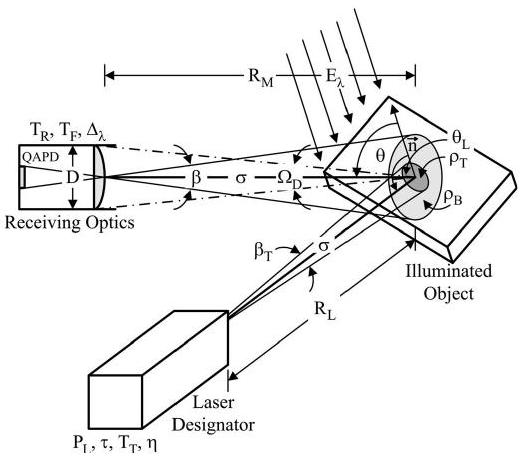
\includegraphics[max width=\textwidth]{5ecfdecb1168916efbeaf9054b715324-02}

Fig. 1. Geometry of the laser transmitter and the receiving optics.

reflector is assumed, which is reflected as a Lambertian source [1]. It is also assumed that the whole laser beam falls on the surface of the illuminated object.

\section{A. Background Power}
The optical power of background \(P_{B}\), which is received at the input of a PSOR, is given by [1]
\[
P_{B}=L_{\lambda} G T_{R} T_{F} \tau_{a t} \Delta_{\lambda}
\]
where \(L_{\lambda}\) is the solar spectral radiance at the object site, \(G\) is the geometrical factor, \(T_{R}\) is the receiving optics transmission coefficient, \(T_{F}\) is the optical filter transmission coefficient, \(\tau_{a t}\) is the transmission coefficient of the atmosphere, and \(\Delta_{\lambda}\) is the optical spectral filter bandwidth. Geometrical factor \(G\) is defined as a factor of the radiation exchange of two small areas, i.e.,
\[
G=\frac{A_{D} \cos \theta \cdot A_{R} \cos \theta_{p o}}{R_{M}^{2}}
\]
where \(A_{D}\) is the area of the detector footprint at the background, \(A_{R} \cos \theta_{p o}\) is the effective area of the optical receiver, \(\theta\) is the angle between the object surface normal and the line joining the object and receiver centers, \(\theta_{p o}\) is the angle between the receiver surface normal and the line joining the object and receiver centers \(\left(\theta_{p o}=0\right.\) because, in the case of good positioning and tracking, the receiving optics is always directed toward the object), and \(R_{M}\) is the distance between the object and the optical receiver.

The solar spectral radiance \(L_{\lambda}\), which is induced by the solar radiation of a diffuse reflector for a specific wavelength \(\lambda\), is given by [1]
\[
L_{\lambda}=\frac{E_{\lambda} \rho_{B}}{\pi}
\]
where \(E_{\lambda}\) is the solar spectral irradiance, and \(\rho_{B}\) is the background reflectance. The atmosphere transmission coefficient \(\tau_{a t}\) is given by
\[
\tau_{a t}=e^{-\sigma R_{M}}
\]
where \(\sigma\) is the atmospheric extinction coefficient. After combining with (2)-(4), the background power given in (1) becomes
\[
P_{B}=\frac{\pi}{16} E_{\lambda} \Delta_{\lambda} \rho_{B} \beta^{2} D^{2} T_{R} T_{F} e^{-\sigma R_{M}} \cos \theta
\]
where \(\beta\) is the receiving optics field of view, and \(D\) is the receiving optics aperture diameter.

\section{B. Signal Power}
The received optical signal power \(P_{S}\) of the reflected laser radiation from the illuminated object, in the case when the area of the laser beam is smaller than the area of the object, is given by [1]
\[
P_{S}=L_{T} A_{T} \Omega_{D} T_{R} T_{F} e^{-\sigma R_{M}} \cos \theta
\]
where \(L_{T}\) is the spectral radiance of the reflected radiation from the object, \(A_{T}\) is the area of the laser spot on the object, and \(\Omega_{D}\) is the solid angle that is subtended by the optical receiver aperture. The spectral radiance \(L_{T}\) is given by
\[
L_{T}=\frac{4 P_{L} T_{T} \eta \rho_{T} e^{-\sigma R_{L}} \cos \theta_{L}}{\pi^{2} \beta_{T}^{2} R_{L}^{2}}
\]
where \(P_{L}\) is the laser peak power, \(T_{T}\) is the transmission coefficient of transmitting optics, \(\eta\) is the transmitting optics collection efficiency, \(\rho_{T}\) is the target reflectance, \(\theta_{L}\) is the angle between the object surface normal and the laser beam, \(\beta_{T}\) is the laser beam divergence angle, and \(R_{L}\) is the distance between the laser and the object. For the surface \(A_{T}\) of the laser spot on the object, the following is valid:
\[
A_{T}=\frac{\pi R_{L}^{2} \beta_{T}^{2}}{4 \cos \theta_{L}}
\]
and for the solid angle \(\Omega_{D}\)
\[
\Omega_{D} \approx \frac{\pi D^{2}}{4 R_{M}^{2}}
\]
Combining (7)-(9) with (6), we finally obtain the following for the received signal optical power \(P_{S}\) :
\[
P_{S}=\frac{D^{2}}{4 R_{M}^{2}} P_{L} \rho_{T} T_{T} \eta T_{R} T_{F} e^{-\sigma\left(R_{L}+R_{M}\right)} \cos \theta
\]

\section{PSOR}
Here, the principles of the angles of azimuth and elevation measurement using the PSOR and the AQPD in pulsed laser tracking systems will be explained. Fig. 2 shows the arrangement of the key optical elements and geometrical parameters of the AQPD in the PSOR.

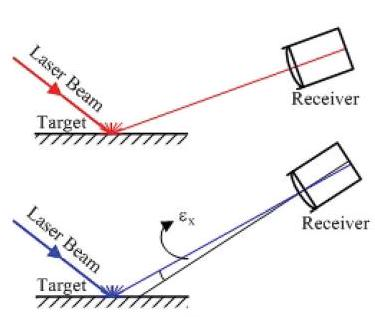
\includegraphics[max width=\textwidth]{5ecfdecb1168916efbeaf9054b715324-03}

(a) Fig. 2. PSOR and AQPD.

The purpose of the optical receiver, which is shown in Fig. 2(a), is to collect the reflected optical energy from the illuminated object. The planoconvex lens, which is placed at the input of the optical receiver, collects the incoming optical energy on the AQPD. To minimize the error, the planoconvex aspherical lens is mostly used because of its minimal spherical aberration coefficient. By using such a lens, the most uniform distribution of the irradiance on the AQPD is achieved. The AQPD is located behind the lens at a distance \(d\) from it. Fig. 2(b) gives an example of the AQPD that is located in front of the focal plane, e.g., \(d<f\), where \(f\) is the focal length of the lens. As the AQPD is not placed at the focal plane, a light spot with an approximately uniform distribution of irradiance is formed on its surface. The radius of the light spot is equal to \(r_{0}\). From the well-known geometrical relations, the following equation for the spot radius is obtained:
\[
r_{0}=\frac{D|f-d|}{2 f}
\]
where \(D\) is the diameter of the lens, \(f\) is the focal length, and \(d\) is the distance between the lens and the AQPD.

When the optical axis and the line object-receiver are not collinear, the light reflected from the object comes with relatively small angle inclination \(\varepsilon_{x}\) toward the optical axis. The center of a light spot that is formed in such a way is moved a distance \(x\) about the center of the AQPD, as shown in Fig. 2(b). As the angle \(\varepsilon_{x}\) is small \(\left(\varepsilon_{x} \ll 1\right)\), it is easy to show that the light spot radius does not significantly change with the light spot movement across the AQPD. Everything that is mentioned\\

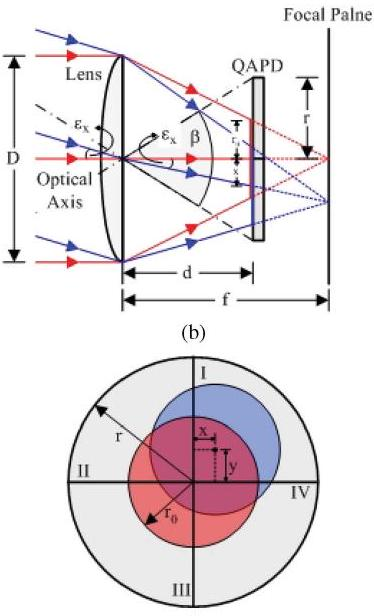
\includegraphics[max width=\textwidth]{5ecfdecb1168916efbeaf9054b715324-03(1)}

©

above is also valid for the second plane, i.e., for the angle \(\varepsilon_{y}\) and for the distance \(y\). Assuming that the reflected optical radiation is uniform, the uniform light spot on the \(A Q P D\) is obtained, as is shown in Fig. \(2(\mathrm{c})\). Two cases are shown in this figure. The first case is when the optical axis and the line object-receiver are collinear. In that case, the light spot center is at the AQPD center. In the second case, the optical axis and the line object-receiver are not collinear, and the light spot is moved about the AQPD center, where \(x\) and \(y\) are the displacements of the light spot along the \(x\) - and \(y\) -axes, respectively.

When the centers of the light spot and the \(A Q P D\) are matched, all four photodiodes are illuminated with the same amount of optical radiation; therefore, all four photodiode currents are the same. When the light spot center is moved, the optical power is divided into four different parts; therefore, the currents of each photodiode are different. By processing these currents, it is possible to obtain the estimation of the distances \(x\) and \(y .\) Based on the determined distances, it is possible to obtain the values of angle displacements \(\varepsilon_{x}\) and \(\varepsilon_{y}\) as
\[
\varepsilon_{x}=\arctan \frac{x}{d} \approx \frac{x}{d}, \quad \varepsilon_{y}=\arctan \frac{y}{d} \approx \frac{y}{d} \text { . }
\]
As can be seen from (12), angles \(\varepsilon_{x}\) and \(\varepsilon_{y}\) are directly proportional to the displacements of light spot centers \(x\) and \(y\), respectively, but only when the following relations are valid: \(|x| \ll d\) and \(|y| \ll d\)

One of the most important parameters of the PSOR is the field-of-view \(\beta\), for which \(\beta=2 \arctan (r / d) \approx 2 r / d\) is valid, where \(r\) is the AQPD radius. The maximum range of the measured angles \(\left(\varepsilon_{x, y}\right)_{\max }\) is equal to half of the field of view, i.e., \(\left(\varepsilon_{x, y}\right)_{\max }=\beta / 2 \approx r / d\). According to this, one can pay special attention to defining the minimal allowed value of the receiver field of view under which the system for positioning and tracking can function correctly. Otherwise, in certain situations, the PSOR can lose the object, which can be critical, particularly in systems such as laser-guided missiles.

\section{A. Light Spot Displacement Measurement}
Direct measurements of displacements \(x\) and \(y\) by processing signals from the AQPD are not possible. By measuring the signals, it is possible to determine the ratios of displacements and the light spot radius, e.g., \(x / r_{0}\) and \(y / r_{0}\). To determine these relations, it is essential to know the irradiance distribution on the AQPD surface. Here, it is assumed that the distribution is uniform. The exact measurements of the ratios \(x / r_{0}\) and \(y / r_{0}\) are not possible, and only the estimations can be made with the following equations [3]:
\[
\begin{array}{l}
\hat{x}_{r}=\frac{\left(I_{\mathrm{I}}+I_{\mathrm{IV}}\right)-\left(I_{\mathrm{II}}+I_{\mathrm{III}}\right)}{\left(I_{\mathrm{I}}+I_{\mathrm{IV}}\right)+\left(I_{\mathrm{II}}+I_{\mathrm{III}}\right)} \\
\hat{y}_{r}=\frac{\left(I_{\mathrm{I}}+I_{\mathrm{II}}\right)-\left(I_{\mathrm{III}}+I_{\mathrm{IV}}\right)}{\left(I_{\mathrm{I}}+I_{\mathrm{II}}\right)+\left(I_{\mathrm{III}}+I_{\mathrm{IV}}\right)}
\end{array}
\]
where \(\hat{x}_{r}\) and \(\hat{y}_{r}\) are the estimated values of the ratios \(x / r_{0}\) and \(y / r_{0}\), respectively, and \(I_{\mathrm{I}}, I_{\mathrm{II}}, I_{\mathrm{III}}\), and \(I_{\mathrm{IV}}\) are the \(\mathrm{AQPD}\) peak currents. For these currents, \(I_{K}=M R_{K} P_{K}\) is valid, where \(M\) is the avalanche photodiode amplification, \(R_{K}\) is the photodiode conversion factor, and \(P_{K}\) is the AQPD peak optical power \((K=\mathrm{I}, \mathrm{II}, \mathrm{III}\), and \(\mathrm{IV})\). Finally, from (13), the following is obtained for the \(x\) -axis:
\[
\hat{x}_{r}=\frac{\left(P_{\mathrm{I}}+P_{\mathrm{IV}}\right)-\left(P_{\mathrm{II}}+P_{\mathrm{III}}\right)}{\left(P_{\mathrm{I}}+P_{\mathrm{IV}}\right)+\left(P_{\mathrm{II}}+P_{\mathrm{III}}\right)} .
\]
If the irradiance on the AQPD surface is uniform, then for the AQPD powers, the following can be stated: \(P_{K}=E_{0} S_{K}\), where \(E_{0}\) is the irradiance at the AQPD surface, and \(S_{K}\) is the area of the illuminated part of the \(K\) th quadrant of the AQPD. Considering this, we can write [4]
\[
\hat{x}_{r}=\frac{\left(S_{\mathrm{I}}+S_{\mathrm{IV}}\right)-\left(S_{\mathrm{II}}+S_{\mathrm{III}}\right)}{\left(S_{\mathrm{I}}+S_{\mathrm{IV}}\right)+\left(S_{\mathrm{II}}+S_{\mathrm{III}}\right)}
\]
This is the most common case in pulsed laser-tracking systems. Now, it is important to find the range of displacements \(x\) and \(y\) for which the whole light spot is located at the AQPD surface. This will provide relatively good linear dependence of \(x\) and \(y\) and the measured values at the output of the AQPD. The whole light spot is on the AQPD surface if the following relation is fulfilled: \(\sqrt{x^{2}+y^{2}}+r_{0} \leq r\). This inequality yields to \(|x| \leq r-r_{0}\) and \(|y| \leq r-r_{0} .\) For the angle range based on (12), the following is valid: \(\left|\varepsilon_{x}\right| \leq\left(r-r_{0}\right) / d\) and \(\left|\varepsilon_{y}\right| \leq\) \(\left(r-r_{0}\right) / d\). According to the angle range requirements, the parameters of the AQPD, such as the light spot radius \(r_{0}\) and the distance between the AQPD and the lens \(d\), should be determined. To provide good linearity, all four photodiodes must be illuminated. This is fulfilled if \(|x| \leq r_{0}\) and \(|y| \leq r_{0}\). Based on these inequalities, the optimal value of the light

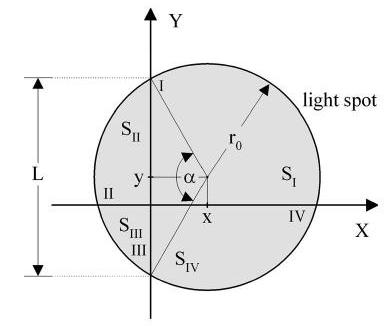
\includegraphics[max width=\textwidth]{5ecfdecb1168916efbeaf9054b715324-04}

Fig. 3. Geometry of the light spot on the AQPD.

spot radius is obtained when both of these two inequalities are fulfilled at the same time, and this is when the following is satisfied: \(r_{0}=r-r_{0}\). This yields to the optimal light spot radius of \(r_{0}=r / 2\).

To find the relations between the light spot displacements and the measured values, it is necessary to determine the illuminated areas of the AQPD \(S_{K}\), where \(K=\mathrm{I}, \mathrm{II}, \mathrm{III}\), and IV. For these areas, from Fig. 3 , it can be written that
\[
\begin{aligned}
S_{\mathrm{I}}+S_{\mathrm{IV}} &=r_{0}^{2} \pi-\left(S_{\mathrm{II}}+S_{\mathrm{III}}\right) \\
S_{\mathrm{II}}+S_{\mathrm{III}} &=r_{0}^{2} \pi \frac{\alpha}{2 \pi}-\frac{1}{2} L x
\end{aligned}
\]
where \(\alpha\) and \(L\) are the geometrical parameters that are shown in Fig. 3. For angle \(\alpha\), the following is valid: \(\alpha=2 \arccos \left(x / r_{0}\right)\); for length \(L, L=2 r_{0} \sin (\alpha / 2) .\) By substituting the last two equations in (16), the following is obtained:
\[
S_{\mathrm{II}}+S_{\mathrm{III}}=r_{0}^{2}\left[\arccos \left(\frac{x}{r_{0}}\right)-\frac{x}{r_{0}} \sqrt{1-\left(\frac{x}{r_{0}}\right)^{2}}\right]
\]
Combining (15)-(17), finally, for \(\hat{x}_{r}\), we have the following:
\[
\hat{x}_{r}=1-\frac{2}{\pi}\left[\arccos \left(\frac{x}{r_{0}}\right)-\frac{x}{r_{0}} \sqrt{1-\left(\frac{x}{r_{0}}\right)^{2}}\right]
\]
If we assume that the displacements are much smaller values with regard to the light spot radius, i.e., \(x \ll r_{0}\), we have
\[
\hat{x}_{r} \approx \frac{4}{\pi} \frac{x}{r_{0}}=S_{\mathrm{QPD}} x
\]
where \(S_{\mathrm{QPD}}\) is the AQPD incremental sensitivity. In the case of the irradiance uniform distribution, \(S_{\mathrm{QPD}}=4 / \pi r_{0}\). Based on (19), we can obtain the estimated value of the light spot displacement \(\hat{x}\), for which we can write
\[
\hat{x}=\frac{\pi}{4} r_{0} \hat{x}_{r}=K_{\mathrm{QPD}} \hat{x}_{r}
\]
where \(K_{\mathrm{QPD}}=1 / S_{\mathrm{QPD}}=\pi r_{0} / 4\) is the proportional factor between the measured and estimated values of the light spot displacements. As it can be seen from (19), the incremental sensitivity is inversely proportional to the light spot radius, which means that the minimal light spot radius is needed for maximum sensitivity.

\section{B. Noise-Induced Measurement Error}
Noise, which is inherent to any electronic device, is one of the most significant causes of angle measurement error in pulsed laser-tracking systems. According to (13) and taking into consideration the equivalent noise sources, we can write
\[
\hat{x}_{r}=\frac{\left(I_{\mathrm{I}}+I_{\mathrm{nI}}+I_{\mathrm{IV}}+I_{\mathrm{nIV}}\right)-\left(I_{\mathrm{II}}+I_{\mathrm{nII}}+I_{\mathrm{III}}+I_{\mathrm{nIII}}\right)}{\left(I_{\mathrm{I}}+I_{\mathrm{nI}}+I_{\mathrm{IV}}+I_{\mathrm{nIV}}\right)+\left(I_{\mathrm{II}}+I_{\mathrm{nII}}+I_{\mathrm{III}}+I_{\mathrm{nIII}}\right)}
\]
where \(I_{n i}\) is the equivalent noise current of the \(i\) th photodiode. If we adopt \(U=I_{\mathrm{I}}+I_{\mathrm{IV}}\) and \(V=I_{\mathrm{II}}+I_{\mathrm{III}}\), as well as \(U_{n}=\) \(I_{\mathrm{nI}}+I_{\mathrm{nIV}}\) and \(V_{n}=I_{\mathrm{nII}}+I_{\mathrm{nIII}}\), we will obtain
\[
\hat{x}_{r}=\frac{\left(U+U_{n}\right)-\left(V+V_{n}\right)}{\left(U+U_{n}\right)+\left(V+V_{n}\right)} .
\]
If we rearrange (22) and assuming that \(U_{n}+V_{n} \ll U+V\), we will obtain
\[
\hat{x}_{r} \approx \frac{U-V}{U+V}+2 \frac{V U_{n}-U V_{n}}{(U+V)^{2}}
\]
The first part of (23) represents the mean value of the relative light spot displacement, and the second part represents the random error in the displacement measuring that is caused by noise. For this measurement error \(\hat{x}_{r n}\), we can write
\[
\hat{x}_{r n} \approx \frac{2 V}{(U+V)^{2}} U_{n}-\frac{2 U}{(U+V)^{2}} V_{n}
\]
As the noise sources in each receiving channel are independent, for the variance \(\sigma_{\hat{x}_{r}}^{2}\) of the relative displacement measurement, the following is valid:
\[
\sigma_{\hat{x}_{r}}^{2} \approx \frac{4 V^{2}}{(U+V)^{4}} \sigma_{u}^{2}+\frac{4 U^{2}}{(U+V)^{4}} \sigma_{v}^{2}
\]
where \(\sigma_{u}^{2}\) and \(\sigma_{v}^{2}\) are the variances of \(U_{n}\) and \(V_{n}\), respectively, and \(\sigma_{u}^{2}=\sigma_{v}^{2}=2 \overline{i_{n}^{2}}\), where \(\overline{i_{n}^{2}}\) is the variance of the noise current in each receiving channel. Now, (25) can be rearranged as
\[
\sigma_{\hat{x}_{r}}^{2} \approx 8 \frac{U^{2}+V^{2}}{(U+V)^{4}} \overline{i_{n}^{2}}
\]
As for \(U\) and \(V, S_{S}=U+V\) is valid, where \(S_{S}\) is the signal in the summing channel, and the variance \(\sigma_{\hat{x}_{x}}^{2}\) of the relative displacement measurement becomes
\[
\sigma_{\tilde{x}_{r}}^{2} \approx 8 \frac{U^{2}+\left(S_{S}-U\right)^{2}}{S_{S}^{4}} \overline{i_{n}^{2}}
\]
The variance \(\sigma_{\hat{x}}^{2}\) from (27) has the minimum value for \(U=\) \(S_{S} / 2\) and \(V=S_{S} / 2 .\) Therefore, we can write
\[
\left(\sigma_{\hat{x}_{r}}^{2}\right)_{\min } \approx \frac{4 \overline{i_{n}^{2}}}{S_{S}^{2}}=\frac{1}{\mathrm{SNR}_{\Sigma}}
\]
where \(\mathrm{SNR}_{\Sigma}\) is the SNR in the summing channel. As can be seen, the minimal variance of the relative displacement measurement is achieved when \(U=V=S_{S} / 2\) is valid, i.e., when the light spot center is at the AQPD center. According to (20), for the minimal value of the estimated light spot displacement standard deviation \(\left(\sigma_{\hat{x}}\right)_{\min }\), we have \([6]\)
\[
\left(\sigma_{\hat{x}}\right)_{\min } \approx \frac{\pi}{4} \frac{r_{0}}{\sqrt{\mathrm{SNR}_{\Sigma}}}
\]
The identical expression is valid for the standard deviation \(\left(\sigma_{\hat{y}}\right)_{\min }\) of the estimated displacement along the \(y\) -axis. Based on (12) and (29), for the minimal standard deviation \(\left(\sigma_{\varepsilon_{x}}\right)_{\min }\) of the measured angle, in the case of a uniform irradiance distribution, we have
\[
\left(\sigma_{\varepsilon_{x}}\right)_{\min } \approx \frac{\pi}{4} \frac{r_{0}}{d} \frac{1}{\sqrt{\operatorname{SNR}_{\Sigma}}}
\]
The parameters \(U\) and \(V\) satisfy the following inequalities: \(U \leq S_{S}\) and \(V \leq S_{S}\). Because of this and according to (27), the maximal value of \(\left(\sigma_{\hat{x}}\right)_{\max }\) is achieved when \(U=S_{S}\) and \(V=0\) (or \(V=S_{S}\) and \(U=0\) ) are fulfilled, i.e., when the light spot center is at the measurement span margin \(\left(x=\pm r_{0}\right.\) and/or \(\left.y=\pm r_{0}\right) .\) Therefore, we have
\[
\left(\sigma_{\hat{x}}^{2}\right)_{\max } \approx \frac{2}{\operatorname{SNR}_{\Sigma}}
\]
Identically, the maximal standard deviations of the estimated displacement along the \(x\) -axis \(\left(\sigma_{\hat{x}}\right)_{\max }\) and the measured angle \(\left(\sigma_{\varepsilon_{x}}\right)_{\max }\) are valid, i.e.,

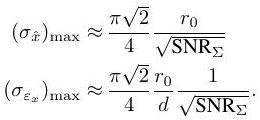
\includegraphics[max width=\textwidth]{5ecfdecb1168916efbeaf9054b715324-05}

The identical expressions are valid for the maximal standard deviation of the estimated displacement along the \(y\) -axis \(\left(\sigma_{\hat{y}}\right)_{\max }\) and the measured angle \(\left(\sigma_{\varepsilon_{v}}\right)_{\max } .\) As can be seen, the maximal standard deviations of measured displacements and angles are \(\sqrt{2}\) times bigger than their minimal values, which does not represent significant enlargement. For us, minimal error in positioning and tracking is important because, when the centers of the light spot and the AQPD are matched, we have good positioning and tracking.

The required span of the measured angles depends on the dynamics of the pulsed laser-tracking system. This measurement span is determined by the receiving optics field-of-view \(\beta\). The receiving optics is designed in such a way as to cover, with its field of view, the complete range of measured angles. According to (30) and the relations between the field of view, the AQPD radius, and the light spot radius, for the noiseinduced angle measurement error \(\sigma_{\varepsilon n}\), we can write
\[
\sigma_{\varepsilon n} \approx \frac{\pi}{16} \beta \frac{1}{\sqrt{\mathrm{SNR}_{\Sigma}}}
\]
As can be seen from (34), it is recommended to choose the value of the field of view as minimal as possible to minimize

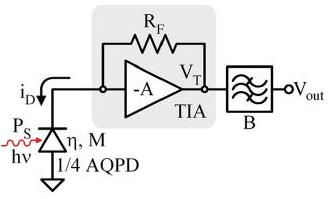
\includegraphics[max width=\textwidth]{5ecfdecb1168916efbeaf9054b715324-06}

Fig. 4. AQPD and TIA.

the angle measurement error. Based on (11) and the relations between the field of view and the remaining optical receiver parameters, and if \(\beta \ll 1\) is satisfied, there is a relation between the AQPD radius and the receiving optics aperture diameter, i.e., \(r \approx \beta f_{n o} D / 2\), where \(f_{n o}\) is the \(f\) -number of the lens, for which \(f_{n o}=f / D\) is valid.

\section{TIA}
In the first stage of the analog signal processing chain from the AQPD, TIAs have two main functions. The first is to filter the noises at their inputs, and the second is to amplify the current signals from the AQPD. At these amplifiers, the current signals at the AQPD are converted into voltage signals to be more suitable for further analog signal processing. The optimization of these amplifiers is essential because it can be the main limiting factor of the whole receiving channel. The electrical scheme of the TIA and the AQPD is shown in Fig. 4 with all the relevant elements.

The voltage signal at the TIA output \(V_{T}\) is equal to \(V_{T}=\) \(R_{F} i_{D}\), where \(R_{F}\) is the resistance of the feedback resistor. Furthermore, this signal is processed by the bandpass filter with the bandwidth equal to \(B\). The function of this filter is to limit the noise level at the TIA output. The bandwidth \(B\) must provide, on one hand, the undisturbed passing through of the useful signal and, on the other hand, the maximal noise filtering. These two conflict requirements can be resolved by choosing the minimal value for bandwidth \(B\), which can provide complete reconstruction of an input signal. This minimal value is equal to \(B \approx 0.35 / t_{r}\), where \(t_{r}\) is the rise time of an input signal, which is defined as \(t_{r}=t_{90 \%}-t_{10 \%}\), where \(t_{90 \%}\) and \(t_{10 \%}\) are the times when the signal is at its \(90 \%\) and \(10 \%\) from its maximal value, respectively. In the case when we have a Gaussian pulse, which is satisfied when the Q-switched Nd:YAG laser is used as a designator, with full-width at half-maximum (FWHM) equal to \(\tau\), we have \(t_{r}=0.716 \tau\) and \(B \approx 0.49 / \tau\).

To determine the angle measurement error, first, we must calculate \(\mathrm{SNR}_{\Sigma}\) in the summation channel. For that reason, it is necessary to determine the equivalent input noise current in each channel. Fig. 5 shows the optimal structure of the TIA [9], with all relevant parameters for determining the equivalent input noise current in one channel. \(\mathrm{SNR}_{\Sigma}\) in the summation channel is equal to
\[
\mathrm{SNR}_{\Sigma}=\frac{I_{S}^{2}}{4 \overline{i_{n}^{2}}}
\]
where \(I_{s}=R_{k} M P_{s}\), and the equivalent noise current \(\overline{i_{n}^{2}}\) is given by [10]
\[
\overline{i_{n}^{2}}=B\left[\overline{i_{n D}^{2}}+\overline{i_{n J}^{2}}+\frac{4 k T}{R_{F}}+\frac{4 \pi^{2}}{3} \overline{e_{n J}^{2}}\left(C_{D}+C_{G}\right)^{2} B^{2}\right]
\]
where \(\overline{i_{n D}^{2}}\) is the avalanche photodiode noise current for which we have
\[
\overline{i_{n D}^{2}}=2 q\left[I_{D R}^{S}+\left(I_{D R}^{V}+I_{B G}+\frac{I_{S}}{4}\right) M^{2} F(M)\right]
\]
where \(q\) is the electron charge, \(I_{D R}^{S}\) is the dark surface current, \(I_{D R}^{V}\) is the dark bulk current, \(I_{B G}=R_{k} P_{B G} / 4\) is the background current, and \(F(M)=M^{n}\) is the avalanche photodiode excess noise factor. The equivalent noise current of the input transistor \(J\), i.e., \(\overline{i_{n . J}^{2}}\), can be neglected because a GaAs MESFET is used as the first stage in the TIA. For equivalent input voltage noise \(\overline{e_{n J}^{2}}\) of a MESFET, we have
\[
\overline{e_{\mathrm{nJ}}^{2}}=\frac{4 \Gamma k T}{g_{m}}
\]
where, for a GaAs MESFET, \(\Gamma=1.5\) is valid, \(k\) is the Boltzmann constant, \(T\) is the absolute temperature, and \(g_{m}\) is the transconductance of an input transistor. In (38), we have omitted the flicker noise because it is dominant only on relatively low frequencies.

In (36), \(C_{D}\) is the AQPD segment capacitance, and \(C_{G}=\) \(C_{G S}+C_{G D}\) is the input capacitance of the TIA, where \(C_{G S}\) and \(C_{G D}\) are the capacitances between the gate and the source and between the gate and the drain of the MESFET, respectively.

Based on the above analysis, it can be noticed that there is an optimal value of avalanche photodiode amplification \(M_{\mathrm{opt}}\), for which the maximal SNR in the summation channel is gained. This optimal value is equal to
\[
M_{\mathrm{opt}}=\left[\frac{2 q I_{D R}^{S}+\frac{4 k T}{R_{F}}+\frac{4 \pi^{2}}{3} \overline{e_{\mathrm{nJ}}}^{2}\left(C_{D}+C_{G}\right)^{2} B^{2}}{n q\left(I_{D R}^{V}+I_{B G}+\frac{I_{S}}{4}\right)}\right]^{\frac{1}{2+n}}
\]
On the other hand, the transconductance of MESFET \(g_{m}\) and of input capacitance \(C_{G}\) are connected with \(g_{m}=K_{J} C_{G}\), where the constant \(K_{J}\) depends on the MESFET channel length. For a MESFET with a \(1-\mu \mathrm{m}\) channel length, \(K_{J} \approx\) \(90 \mathrm{mS} / \mathrm{pF}\) is valid. It is possible to select the optimal MESFET channel width that provides the minimal value of the equivalent voltage noise at the preamplifier input. The channel width is selected to fulfill the relation \(C_{D}=C_{G}\)

The AQPD parameters, such as the segment capacitance, the dark surface current, and the dark bulk current, depend on the AQPD radius in such a way that the segment capacitance and the dark bulk current depend on the segment area, and the dark surface current depends on the segment arc length along the AQPD circumference [1], [13]. The relations between these parameters are \(C_{D}=K_{C} \pi r^{2} / 4, I_{D R}^{S}=K_{S} \pi r / 2\), and

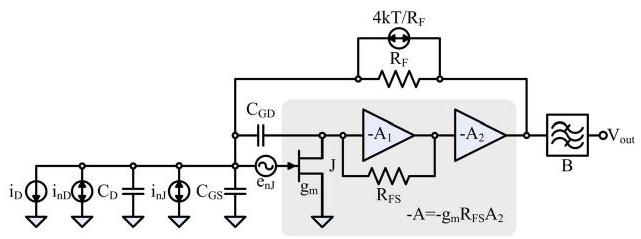
\includegraphics[max width=\textwidth]{5ecfdecb1168916efbeaf9054b715324-07}

Fig. 5. Optimal structure of the TIA.

\(I_{D R}^{V}=K_{V} \pi r^{2} / 4\), where \(K_{C}, K_{S}\), and \(K_{V}\) are the corresponding constants that depend on the used technology. To minimize the overall noise, it is important to select the technology that will keep those constants as minimal as possible. It is also important that the AQPD radius should be as minimal as possible; however, there are some limitations, such as the minimal value of the receiving optics field of view. In that case, it is necessary to select the lens that has a minimal value of the \(f\) -number.

\section{ATMOSPHERE-INDUCED ERRORS}
Atmospheric turbulence causes phenomena commonly referred to as beam wander, scintillation, and beam breathing, according to the effect that is produced on the beam spot as seen on the screen after traveling through a turbulent atmosphere. Beam wander means random changes in the position of the beam spot on the screen, in the scintillation illumination fluctuations within the beam, and also in the breathing expansion and contraction of the spot beyond the dimensions that are predicted by its geometry and diffraction. These effects are caused by index-of-refraction inhomogeneities, which mainly arise from spatial temperature differences within the atmosphere.

A turbulent atmosphere can be thought to be composed of cells of various sizes that differ in their index of refraction. As these cells move across a beam of light, they cause the effects described above. According to this “frozen” atmosphere assumption, the velocity and the direction of this uniform motion are determined by the mean wind speed.

Depending on the dominant cell size and the beam diameter, turbulent cells affect light propagation in different ways. Cells that are larger than the beam diameter act like weak lenses and deflect the beam as a whole in a random way (angle of wavefront), leaving its irradiance distribution unaltered essentially (beam wander); however, when the cell size is smaller than the diameter of the beam, refraction and diffraction take place, and the irradiance profile of the beam breaks up into small bright and dark areas as a result of refracted and diffracted wavefront interference (scintillation). Depending on the relative strength of the turbulence, either of the effects may be observed, or both may be observed simultaneously. The dominant effect is beam wander in weak turbulence and scintillation in strong turbulence [14].

The strength of the atmospheric turbulence is described by the refractive index structure coefficient \(C_{n}\), which is, basi- cally, a measure of the spatial gradient of the refractive index (temperature) within the atmosphere. From the sensor point of view, the strength of the turbulence also depends on the length of the path that the light traverses. The strength of the pathintegrated turbulence is given by the spherical wave coherence length \(\rho_{0}=\left(0.545 \kappa^{2} R C_{n}^{2}\right)^{-3 / 5}[5]\), where \(\kappa=2 \pi / \lambda\), and \(R\) is the distance that the beam travels in a turbulent atmosphere. This describes the amount of scattering that is caused by the atmospheric turbulence and is used to determine whether the turbulence in a particular case is considered weak or strong. Turbulence is considered weak if \(\rho_{0}\) is larger than the diffraction patch size \(\sqrt{R \lambda}\); otherwise, it is considered strong [15]. The following classification of the turbulence strength can also be found: \(C_{n}=8 \times 10^{-9} \mathrm{~m}^{-1 / 3}\) for weak turbulence, \(C_{n}=4 \times\) \(10^{-8} \mathrm{~m}^{-1 / 3}\) for medium turbulence, and \(C_{n}=5 \times 10^{-7} \mathrm{~m}^{-1 / 3}\) for strong turbulence [16].

The effect of the atmospheric turbulence on beam propagation is a result of complicated phenomena. In certain cases, however, it can be satisfactorily estimated using simple equations. Geometric optical formulation, for example, can be successfully used to predict large-scale effects such as angleof-arrival fluctuations or beam wander [15], [17]. This presupposes, however, that the beam diameter \(\phi\) should not be markedly altered by diffraction or by scattering due to the atmospheric turbulence. The first condition is fulfilled if the measurement distance is within the Fresnel diffraction range \((\phi>\sqrt{R \lambda})\), and the second condition is fulfilled if the pathintegrated turbulence is weak \(\left(\rho_{0}>\sqrt{R \lambda}\right)[15]\).

The various mechanisms by which the measurement precision of a reflected beam sensor is affected include angular fluctuations in the wavefront, irradiance fluctuations at a misfocused receiver aperture, and irradiance fluctuations. Simple equations are presented below to estimate the magnitude of the above effects. The derivations were performed by combining the results of several publications.

\section{A. Angle-of-Arrival Fluctuations}
The angle of arrival is the average tilt of a wavefront across the receiver aperture and is, thus, the same as the angle (direction) of the received beam. A general form for the equation required to estimate the variance of angle-of-arrival fluctuations \(\sigma_{\varepsilon a}^{2}\) is given by \([5]\)
\[
\sigma_{\varepsilon a}^{2}=\varphi C_{n}^{2} D^{-\frac{1}{3}} R
\]
where \(\varphi\) is a constant, \(D\) is the aperture diameter, and \(R\) is the distance that the beam travels in a turbulent atmosphere before reaching the aperture. Based on [5], the constant \(\varphi\) is equal to \(\varphi \approx 0.79\). As the reflected beam travels the path from the object to the receiving optics, we have \(R=R_{M}\). Therefore, for the variance of the angle-of-arrival fluctuations, we have
\[
\sigma_{\varepsilon a}^{2}=\varphi C_{n}^{2} D^{-\frac{1}{3}} R_{M}
\]

\section{B. Effect of Irradiance Fluctuations}
Irradiance fluctuations that are caused by the atmospheric turbulence affect precision if the receiver is misfocused. The atmospheric turbulence causes the received irradiance to fluctuate across the receiver aperture. These fluctuations cause no problems in a focused case because each elemental area of the receiver images the light collected by it onto the entire image spot. In this situation, the irradiance fluctuations that are related to the elemental area change the irradiance of the image spot, uniformly leaving its centroid unaltered. In a misfocused receiver, however, the irradiance fluctuations across the receiver aperture are directly projected on the light spot on the AQPD surface. These spatially uncorrelated fluctuations then cause variation in the light spot centroid and affect the measurement precision. In the case of a misfocused AQPD receiver, the standard deviation \(\sigma_{\varepsilon i}\) of the measured object position due to irradiance fluctuations is given by [5]
\[
\sigma_{\varepsilon i} \approx \frac{\pi}{8} \frac{r_{0}}{d} \sqrt{\frac{1-c_{c}}{\mathrm{SFR}}}=\frac{\pi}{32} \beta \sqrt{\frac{1-c_{c}}{\mathrm{SFR}}}
\]
where \(c_{c}\) is the correlation coefficient of the irradiance fluctuations between crosswise quadrants of the circular receiver aperture, and SFR is the signal-to-fluctuation ratio that is related to one quadrant of the receiver aperture, which is defined as the average signal power divided by the root-mean-square value of its fluctuations [22].

In the case of narrow-band laser irradiance, the spatial correlation depends on the effective distance of the crosswise receiver aperture quadrants in relation to the Fresnel zone size \(\sqrt{R \lambda}\), and the SFR depends on the path-integrated turbulence strength and the averaging that is provided by the receiver aperture quadrant [23]. It can be concluded from [17] that if the receiver is directly illuminated by a point source, and two receiver points have lateral separation that is larger than about \(D_{K} \approx 0.6 \sqrt{R_{M} \lambda}, c_{c}\) is essentially zero. This means that the irradiance fluctuations of crosswise receiver quadrants should be uncorrelated when practical aperture sizes of a few centimeters and measurement distances of up to a couple of hundreds of meters are used. In the case of pulsed laser-tracking systems for approximately \(R_{M} \approx 10 \mathrm{~km}\) and \(\lambda=1.064 \mu \mathrm{m}\), the minimal lateral separation between two receiver points, for which we have a correlation coefficient that is approximately equal to zero, is approximately \(6 \mathrm{~cm}\). As the receiver aperture could be several centimeters in diameter, we can assume that \(c_{c} \neq 0\). Moreover, as it is valid that for \(D=0\), the correlation coefficient is \(c_{c} \approx 1\), and for \(D \geq D_{K}\), the correlation coeffi- cient is \(c_{c} \approx 0\), we can make the assumption that the correlation coefficient \(c_{c}\) dependence on the aperture diameter \(D\) is linear. Therefore
\[
c_{c}=\left\{\begin{array}{ll}
1-\frac{D}{D_{K}}, & D \leq D_{K} \\
0, & D>D_{K}
\end{array}\right.
\]
where \(D_{K}=0.6 \sqrt{R_{M} \lambda}\). In the case of the narrow-band irradiance, the SFR can be deduced in the following way. In the weak turbulence, the normalized irradiance variance for a point receiver that is illuminated by a diverging beam is \(\sigma_{I p r}^{2}=\) \(0.496 \kappa^{7 / 6} R_{M}^{11 / 6} C_{n}^{2}[27] .\) This magnitude of fluctuations is reduced by aperture averaging. Therefore, for the normalized irradiance variance \(\sigma_{I e r}^{2}\), we have
\[
\sigma_{\text {Ier }}^{2}=\frac{\sigma_{I p r}^{2}}{A_{\gamma}}
\]
where \(A_{\gamma}\) is given by
\[
A_{\gamma}=1+0.362 \gamma^{-\frac{7}{3}}
\]
and \(\gamma=D / \sqrt{R_{M} \lambda}[27] .\) Finally, for the SFR, we have \(\mathrm{SFR}=1 / \sigma_{\text {Ier }}^{2}\). By combining (42), (44), and (45), we finally obtain the following:
\[
\mathrm{SFR}=\frac{1+0.362\left(\frac{D}{\sqrt{R_{M}} \lambda}\right)^{-\frac{7}{3}}}{0.496 \kappa^{\frac{7}{6}} R_{M}^{\frac{11}{6}} C_{n}^{2}}
\]
Based on (42) and (46), for the standard deviation \(\sigma_{\varepsilon i}\) of measured angles caused by the irradiance fluctuation on the AQPD surface, we have
\[
\sigma_{\varepsilon i}=\frac{\pi}{32} \beta \sqrt{1-c_{c}}\left[\frac{0.496 \kappa^{\frac{7}{6}} R_{M}^{\frac{11}{6}} C_{n}^{2}}{1+0.362\left(\frac{D}{\sqrt{R_{M} \lambda}}\right)^{-\frac{7}{3}}}\right]^{\frac{1}{2}}
\]

\section{TOTAL ANGLE MEASUREMENT ERROR}
There are three main factors that cause the angle measurement error-random noise in the receiver channel, angle-ofarrival fluctuations, and irradiance fluctuations on the AQPD surface. All these measurement errors are characterized by their variances. As these random processes are independent, for the variance \(\sigma_{\varepsilon T O T}^{2}\) of the total angle measurement error, we have
\[
\sigma_{\varepsilon T O T}^{2}=\sigma_{\varepsilon n}^{2}+\sigma_{\varepsilon a}^{2}+\sigma_{\varepsilon i}^{2}
\]
In any control system for automatic positioning and tracking, there is maximal allowed error in angle measurement for which the system is functional. The value of this maximal allowed error depends on the actual system realization. The common accepted value for the maximal allowed standard deviation of this error is 2 mrad. Based on this accepted value, the maximal operating range for positioning and tracking can be defined. In that case, for the maximal range \(R_{D}\) defined the way it is

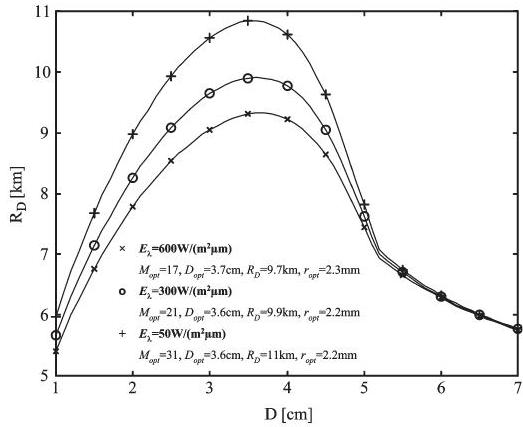
\includegraphics[max width=\textwidth]{5ecfdecb1168916efbeaf9054b715324-09}

Fig. 6. Maximal range \(R_{D}\) dependence on the optical receiver aperture diameter \(D\).

described above, the following is valid: \(R_{D}=R_{M}\left(\sigma_{\varepsilon T O T}=\right.\) \(2 \mathrm{mrad}\) ), where \(R_{M}\left(\sigma_{\varepsilon T O T}=2 \mathrm{mrad}\right)\) is the distance between the illuminated object and the receiver at which the total angle measurement error is equal to \(2 \mathrm{mrad}\).

Fig. 6 shows the dependence of maximal range \(R_{D}\) versus receiver aperture diameter \(D\) for the following parameters: laser peak power \(P_{L}=5\) MW; FWHM of the laser pulse \(\tau=20 \mathrm{~ns}\) (energy per laser pulse is given by \(\left.E_{L} \approx 100 \mathrm{~mJ}\right)\); field of view of the receiving optics \(\beta=10^{\circ}\); MESFET constant \(K_{J}=90 \mathrm{mS} / \mathrm{pF} ;\) MESFET excess noise factor \(\Gamma=1.5\); optical filter spectral bandwidth \(\Delta_{\lambda}=1 \mathrm{~nm} ;\) receiving optics transmission coefficient \(T_{R}=0.9\); optical filter transmission coefficient \(T_{F}=0.4\); refractive index structure coefficient \(C_{n}=\) \(8 \times 10^{-9} \mathrm{~m}^{-1 / 3}\) (this value for the refractive index structure coefficient is taken because it represents the mean value in the case of weak turbulence); avalanche photodiode excess noise factor coefficient \(n=0.4\); transimpedance resistance \(R_{F}=10 \mathrm{k} \Omega\); avalanche photodiode conversion coefficient for unit gain \(R_{k}=0.45 \mathrm{~A} / \mathrm{W}\); avalanche photodiode technology coefficients \(K_{C}=1 \mathrm{pF} / \mathrm{mm}^{2}, K_{S}=3 \times 10^{-8} \mathrm{~A} / \mathrm{mm}\), and \(K_{V}=1 \times 10^{-10} \mathrm{~A} / \mathrm{mm}^{2}[28] ; f\) -number of the aspheric planoconvex lens \(f_{n o}=0.7\); background reflectance \(\rho_{B}=0.4\); target reflectance \(\rho_{T}=0.2\); atmospheric extinction coefficient \(\sigma=0.15 \mathrm{~km}^{-1} ;\) laser-object distance \(R_{L}=2 \mathrm{~km} ;\) the angle between the object surface normal and the line joining the object and receiver centers \(\theta=45^{\circ}\); the transmission coefficient of transmitting optics \(T_{T}=0.9\); transmitting optics collection efficiency \(\eta=0.6\); and absolute temperature \(T=300 \mathrm{~K}\). For the solar spectral irradiance, three values were taken: \(E_{\lambda}=50\), 300, and \(600 \mathrm{~W} /\left(\mathrm{m}^{2} \cdot \mu \mathrm{m}\right)\).

As can be seen from Fig. 6 , there is an optimal value of the receiving optics aperture diameter \(D_{\mathrm{opt}}\) for which the pulsed laser tracking system has the maximal positioning and tracking range. Although we have changed the value of the solar spectral irradiance in the wide range, the optimal value of the receiving optics aperture diameter has changed only slightly. The optimal value of this diameter is in the range of \(3.6-3.7 \mathrm{~cm}\). The optimal avalanche photodiode amplification \(M_{\text {opt }}\) is also changed in the relatively narrow range from 17 to 31 . Concerning the optimal aperture diameter and the minimal allowed field of view, the optimal radius \(r_{\text {opt }}\) of the AQPD was found based on the equation \(r_{\mathrm{opt}} \approx \beta f_{n o} D_{\mathrm{opt}} / 2\) given in Section III-B. Simple calculations give the optimal AQPD radius to be approximately \(r_{\mathrm{opt}} \approx 2.2 \mathrm{~mm}\). Regarding the maximally allowed angle measurement error of about \(2 \mathrm{mrad}\), the maximal range was estimated. From Fig. 6 , it can be seen that the maximal range depends on the solar spectral irradiance and is in the range from 9 to \(11 \mathrm{~km}\).

\section{CONCLUSION}
Concerning the maximal range of positioning and tracking in pulsed laser-tracking systems, the optimal parameters of an optical receiver have been found. It has been shown that there is an optimal receiving optics aperture diameter, which is slightly changed by changing the solar irradiance conditions. The optimal diameter is approximately equal to \(3.6 \mathrm{~cm}\) for a standard set of parameters, as shown in Section \(\mathrm{V}\). This optimal diameter value is in good agreement with the aerodynamical requirements for laser-guided missiles. Also, the optimal value of the AQPD radius has been found to be equal to approximately \(2.2 \mathrm{~mm}\). Taking into consideration all these parameters and regarding the maximally allowed measurement error, the maximal possible range was found to be approximately \(10 \mathrm{~km}\).

\section{ACKNOWLEDGMENT}
The authors would like to thank the encouragement and the support of Prof. A. Mariněić.

\section{REFERENCES}
[1] H. N. Burns, C. G. Christodoulou, and G. D. Boerman, “System design of a pulsed laser range finders,” Opt. Eng., vol. 30, no. 3, pp. 323-329, Mar. \(1991 .\)

[2] Z. Barbaric and M. Nikolic, “Parametrical analysis of pulsed laser rangefinder’s range,” in Proc. XLII ETRAN Conf., Vrnjacka Banja, Serbia, Jun. \(3-5,1998\).

[3] W. L. Wolfe and G. J. Zissis, The Infrared Handbook. Ann Arbor, MI:

Environ. Res. Inst. Michigan, \(1978 .\)

[4] E. O. Doebelin, Measurement Systems Application and Design. New York: McGraw-Hill, \(1990 .\)

[5] L. G. Kazovsky, “Theory of tracking accuracy of laser systems,” Opt. Eng., vol. 22, no. 3, pp. 339-347, May/Jun. \(1983 .\)

[6] A. Mäkynen, “Position-sensitive devices and sensor systems for optical tracking and displacement sensing applications,” Ph.D. dissertation, Dept. Elect. Eng., Univ. Oulu, Oulu, Finland, 2000 .

[7] A. Mäkynen, J. Kostamovaara, and R. Myllylä, “Positioning resolution of the position-sensitive detectors in high background illumination,” IEEE Trans. Instrum. Meas., vol. 45, no. 1, pp. 324-326, Feb. \(1996 .\)

[8] Y. Yanhai, “The design of echo spot and optical focusing in automatic laser tracking,” Opt. Laser Technol., vol. 18, no. 2, pp. \(75-79,1986 .\)

[9] P. W. Young, L. M. German, and \(R\). Nelson, “Pointing, acquisition, and tracking subsystem for space-based laser communications,” Proc. SPIE, vol. 616, pp. \(118-128,1986\).

[10] J. L. Hullett and S. Moustakas, “Optimum transimpedance broadband optical preamplifier design,” Opt. Quantum Electron., vol. 13, no. 1, pp. 65-69, Jan. 1981 .

[11] L. M. Manojlovic, “Analysis and optimization in receiving optical signal from optoelectronic coordinator in pulsed laser tracking systems,” M.S. thesis, Electrotechnical Faculty, Univ. Belgrade, Belgrade, Serbia, \(2003 .\) [12] Z. P. Barbaric and L. M. Manojlovic, “Optimization of optical receiver parameters for pulsed laser tracking systems,” in Proc. 6th Int. Cont. Telecommun. Modern Satell., Cable Broadcast. Service, TELSIKS, 2003 vol. 1, pp. \(192-201\).

[13] H. Ando, H. Kanbe, T. Kimura, T. Yamaoka, and T. Kaneda, "Characteristics of germanium avalanche photodiodes in the wavelength region of \(1-1.6 \mu \mathrm{m}, "\) IEEE J. Quantum Electron., vol. QE-14, no. 11, pp. \(804-809\) Nov. 1978 .

[14] H. Weichel, Laser Beam Propagation in the Atmosphere. Bellingham,

WA: SPIE, 1990, pp. \(45-66 .\)

[15] J. H. Churnside and R. J. Lataitis, Statistics of a Reflected Laser Beam in the Turbulent Atmosphere (Path Correlation). Boulder, CO: Nat. Ocean. Atmos. Admin., Environ. Res. Lab., Wave Propagation Lab., \(1989 .\) NOAA Tech. Memo. ERL WPL-172.

[16] Z. Gossorg, Infrared Thermography-Principles, Techniques, Application.

Moscow, Russia, 1988 . (in Russian).

[17] R. S. Lawrence and J. W. Strohbehn, “A survey of clear-air propagation effects relevant to optical communications,” Proc. IEEE, vol. 58, no. 10 , pp. \(1523-1545\), Oct. \(1970 .\)

[18] T. Chiba, “Spot dancing of the laser beam propagated through the turbulent atmosphere,” Appl. Opt., vol. 10, no. 11, pp. 2456-2461. \(1971 .\)

[19] J. W. Dowling and P. M. Livingston, "Behavior of focused beams in atmospheric turbulence: Measurements and comments on the theory,’ J. Opt. Soc. Amer, vol. 63, no. 7, pp. 846-858, \(1973 .\)

[20] J. H. Churnside and R. J. Lataitis, “Angle-of-arrival fluctuations of a reflected beam in atmospheric turbulence,” \(J .\) Opt. Soc. Amer. \(A, O p t .\) Image Sci., vol. 4, no. 7, pp. 1264-1272, 1987

[21] J. H. Churnside and R. J. Lataitis, "Wander of an optical beam in

the turbulent atmosphere," Appl. Opt., vol. 29, no. 7, pp. 926-930. \(1990 .\)

[22] G. A. Andreev and R. M. Magind, “Influence of intensity fluctuations on the measurement of angular position of radiation source by opticalelectron monopulse method,” Izvestiva Vysshikh Uchebnykh Zavedeni Radiofizika, vol. 15, no. 1, pp. \(55-61,1972 .\)

[23] A. Mäkynen, J. Kostamovaara, and R. Myllylä, “Displacement sensing resolution of position-sensitive detectors in atmospheric turbulence using retroreflected beam,” IEEE Trans. Instrum. Meas., vol. 46, no. 5 pp. 1133-1136, Oct. \(1997 .\)

[24] R. L. Fante, "Electromagnetic beam propagation in turbulent media,

Proc. IEEE, vol. 63, no. 12, pp. \(1669-1692\), Dec. 1975 .

[25] W. A. Coles and R. G. Frechlich, “Simultaneous measurement of angular scattering and intensity scintillation in the atmosphere,” J. Opt. Soc. Amer, vol. 72, no. 8, pp. \(1042-1048,1982\).

[26] J. H. Churnside and J. J. Wilson, "Enhanced backscatter of a reflected

[27] H. Weichel, Laser Beam Propagation in the Atmosphere. Bellingham,

WA: SPIE, 1990 , pp. \(45-66\).

[28] P. E. Webb, R. J. McIntyre, and J. Conardi, "Properties of Avalanche

Photodiodes," RCA, New York, NY, \(1977 .\) Tech. Rep.

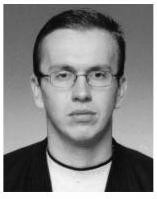
\includegraphics[max width=\textwidth]{5ecfdecb1168916efbeaf9054b715324-10}

Lazo M. Manojlović was born in Vranje, Serbia, on April \(30,1972 .\) He received the B.Sc.E.E. and M.Sc.E.E. degrees in electrical engineering from the University of Belgrade, Belgrade, Serbia, in 1996 and 2003 , respectively.

From 1997 to 1998, he was with the Institute Mihajlo Pupin, Belgrade, as a part of his extended studies, where he worked on the development of applicative software for the text-to-speech synthesis of the Serbian language in C programming language based on diphone concatenation. From 1998 to 2002, he was with the Military Institute of Technology, Belgrade, where he worked on designing and testing several types of ultralow-noise wideband photodiode preamplifiers for quadrant photodetectors and tracking electronic circuits for analog signal processing in pulsed laser tracking systems for laser guidance missiles. From 2002 to 2003, he was with Pupin Telecom DATACOM, Belgrade, where he took part in the design, installation, and commission of the first HFC network for the Cable Distribution Systems in Belgrade, which will provide several services such as cable TV, fast Internet, interactive television, video on demand, and telephony over IP. From 2003 to 2005, he was with the Vienna University of Technology, Vienna, Austria, where he worked on the development of high-precision piezo actuator-based positioning systems. Since 2005, he has been with the Integrated Microsystems Austria GmbH, Wiener Neustadt, Austria, where he is working on the development of different types of fiber-optic sensors. His research interests include interferometry, optical sensing systems, and laser rangefinders.

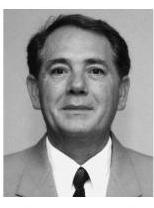
\includegraphics[max width=\textwidth]{5ecfdecb1168916efbeaf9054b715324-10(1)}

Žarko P. Barbarić was born in Knešpolje, Bosnia and Herzegovina, on September \(18,1949 .\) He received the B.Sc.E.E., M.Sc.E.E., and Ph.D. degrees in electrical engineering from the University of Belgrade, Belgrade, Serbia, in 1978,1985, and 1991 , respectively.

From 1978 to 2005, he was with the Electronic Research and Development Division, Military Institute of Technology, Belgrade, where he became a Research and Development Engineer, the Chief of the Electronic Department and Division, and the Project Manager for the Laser Guidance Systems Project. Since 1985, he has been with the Faculty of Electrical Engineering, University of Belgrade, where he is currently a Professor of remote sensing and infrared thermal imaging (thermal vision) with the Department of Telecommunications. He is also an Associate Professor with the Faculty of Technical Sciences, University of Novi Pazar, Novi Pazar, Serbia. He has authored several international papers on infrared thermal imaging (the computer model for the line scanning techniques), statistical properties of infrared imagers, laser-tracking systems. position error estimation for the quadrant photodiode position sensor, etc. His research interests include electrooptical systems for reconnaissance, infrared laser guidance systems, and passive tracking systems.


\end{document}